\documentclass[a4paper]{article}

%\usepackage[document]{ragged2e}
\usepackage{fullpage} % Package to use full page
\usepackage{parskip} % Package to tweak paragraph skipping
\usepackage{tikz} % Package for drawing
\usepackage{amsmath}
\usepackage{hyperref}

\title{Introduction to Intelligent Systems: Assignment 1
\\The Travelling Salesperson Problem}
\author{Damiano Melotti (S3838706)\\Amadeus Beckmann (S3839508) }
\date{\today}

\begin{document}

\maketitle

\section{Introduction}

In our first lecture of the course we discussed the \textsc{TSP}, that given a map with \(N\) cities requires to find the shortest path which visits every city exactly once, starting and ending at the same point. \iffalse It is a NP-hard problem, so unless \(P=NP\), we do not know any deterministic algorithm that runs in polynomial time. \fi

During our lecture we have seen a heuristic algorithm based on a \textbf{greedy} approach. Starting with a random round trip, it tries to improve the path by swapping two cities, comparing the path lengths and replacing the previous one if the total length has decreased. This solution has the limitation of getting stuck at a \textbf{local minimum}, because it never accepts variations that temporarily increase the path length to produce a better result.

To allow for changes that increase the length of the path, in order to leave local minima and get closer to the global minimum, we introduced the \textbf{Metropolis algorithm}. In addiction to the greedy approach, it also accept increasing path lengths with a certain probability. To calculate it we used a parameter \(T\) called \textbf{temperature}, that controls the acceptance rate.

In this assignment we will work with the Metropolis algorithm for \(N=50\) cities at a non-changing temperature \(T\), analysing its behaviour with different values. In the end we will discuss the relation between \(T\) and the mean length \(\langle \mathscr{l} \rangle\) of the path. 


\section{Observations on the Metropolis algorithm}

To examine how the given temperatures change the resulting average path length we created a graph showing the mean path and its variance as a function of temperature.

\begin{figure}[!htbp]
\begin{center}
%\includegraphics[width=7.5cm]{plot1.png}
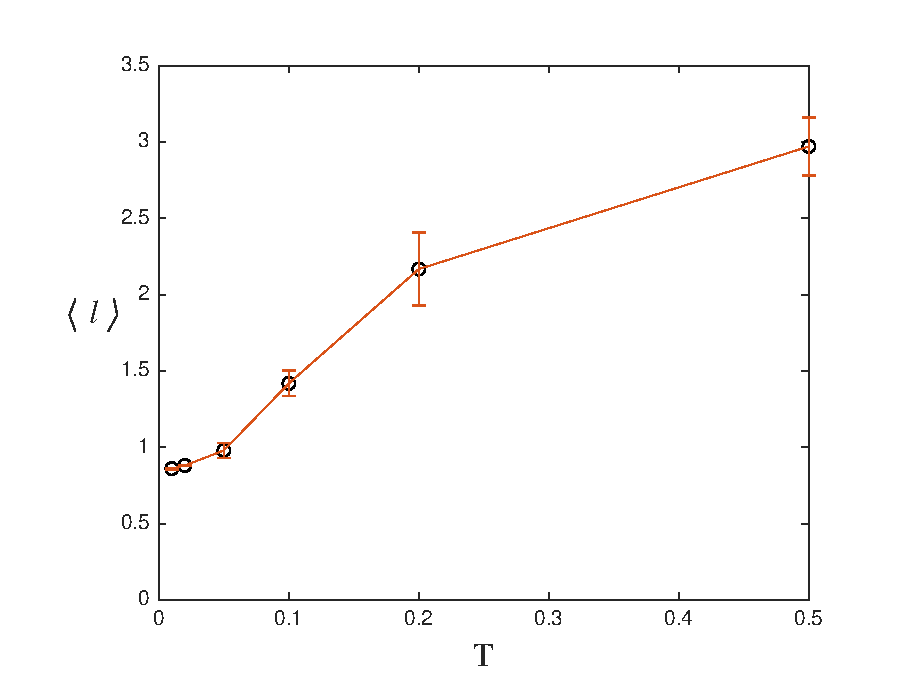
\includegraphics[width=7.5cm]{plot1_v2.eps}
\end{center}
\caption{Mean path lengths and variances for different temperatures}
\end{figure}

Observing this plot we notice that for higher temperatures the mean path lengths also increase because the acceptance rate for new paths that may increase the total length is too high. However, does it also mean that lower temperatures always give better results? And what happens if the temperatures increases further?

The following two plots give a good explanation.

\begin{figure}[!htbp]
  \centering
  \begin{minipage}[b]{7.5cm}
    %\includegraphics[width=\textwidth]{plot2.png}
    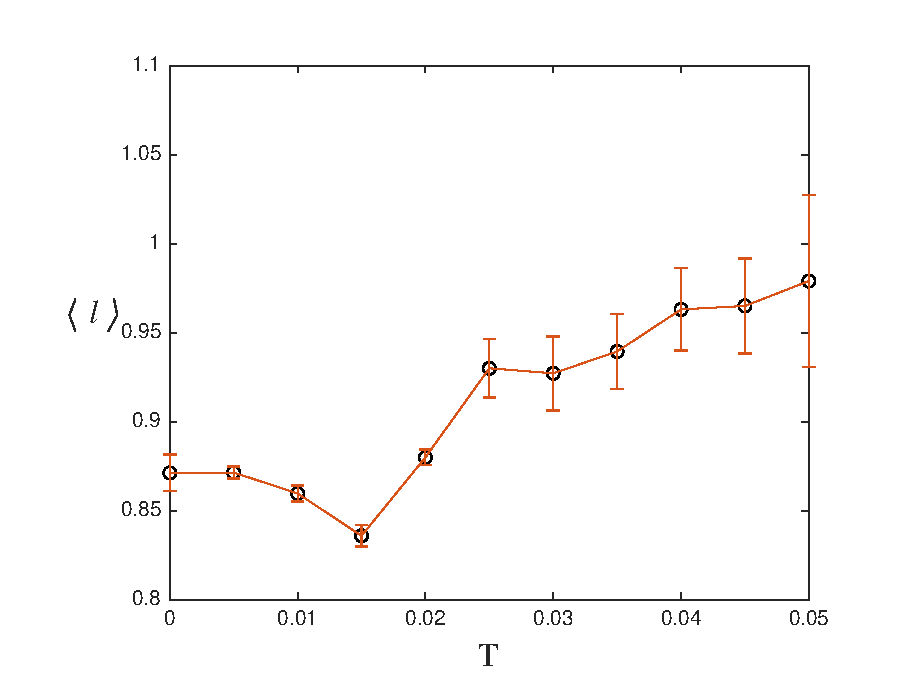
\includegraphics[width=\textwidth]{plot2_v2.eps}
    \caption{Low temperatures}
  \end{minipage}
  \begin{minipage}[b]{7.5cm}
    %\includegraphics[width=\textwidth]{plot3.png}
    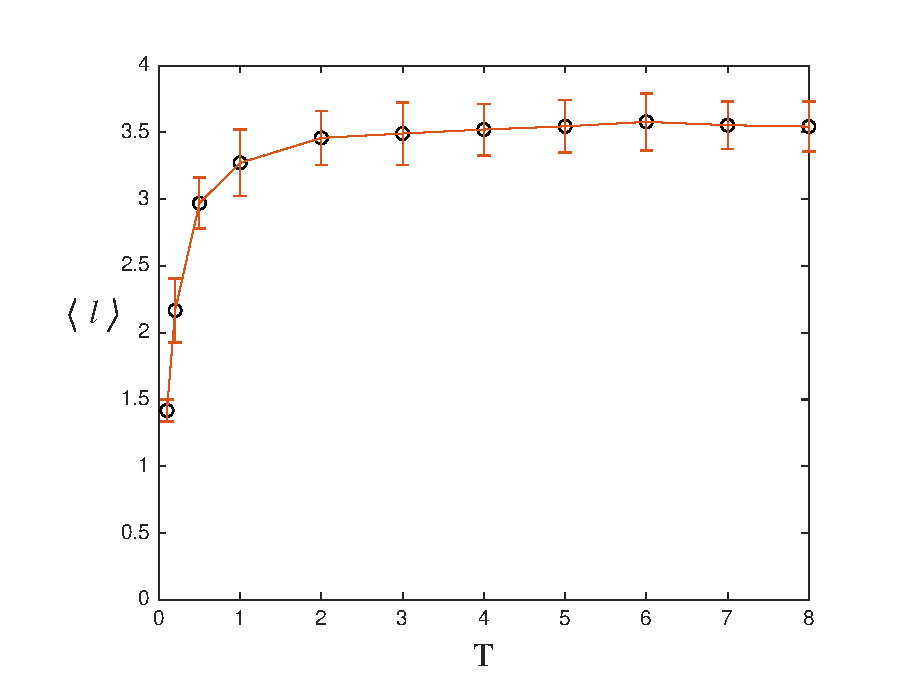
\includegraphics[width=\textwidth]{plot3_v2.eps}
    \caption{High temperatures}
  \end{minipage}
\end{figure}

\textbf{Figure 2} clearly shows an increasing average path length for temperatures lower than 0.01, which apparently is the best value for the temperature in this simulation. Lower values for \(T\) don't allow to accept enough lengths that would increase the final path and therefore produce worse results. We are basically getting closer to the greedy version of the algorithm. \textit{N.B.: To focus on the important part of the plot the \(y\)-axis starts at 0.8.}

\textbf{Figure 3} illustrates that raising temperatures do not cause significant changes in the final length because they lead to an almost random path. As there are many inefficient paths and few good ones, choosing randomly obviously means worse results.

Another consequence of higher temperatures is a higher variance in the path length, because it is more likely to accept a new path that remarkably changes the previous one in terms of discarding a good solution.


\section{Conclusion}

To sum up the Metropolis algorithm for the \textsc{TSP} works better with temperatures close to 0. However it is important to pick the right value, because as shown earlier getting too close to 0 just results in a greedy approach.

As considered during the lecture a possible improvement would be gradually lowering the temperature because allowing to choose a bad path in the beginning but not later can lead to a more refined round trip.

In every case it is advisable to run the algorithm multiple times as the random starting path has a strong influence on the final result.


\end{document}
